A continuación se describe el producto obtenido, siguiendo las diferentes fases de la metodología de trabajo y las herramientas descritas con anterioridad. Además, se indica el código de los inconvenientes que se resuelven expuestos en la \textbf{Sección \ref{sec:Errores_Frecuentes}}.

\paragraph{Autentificación de un usuario en el sistema: } Solicitud de acceso, utilizando credenciales de acceso los cuales son ingresados por el usuario. Si las credenciales son válidas, se redirecciona a las interfaces de la OE interesada o a la del Administrador (vea \textbf{Figura \ref{fig: Login}}).

\begin{figure}[htbp]
    \centering
    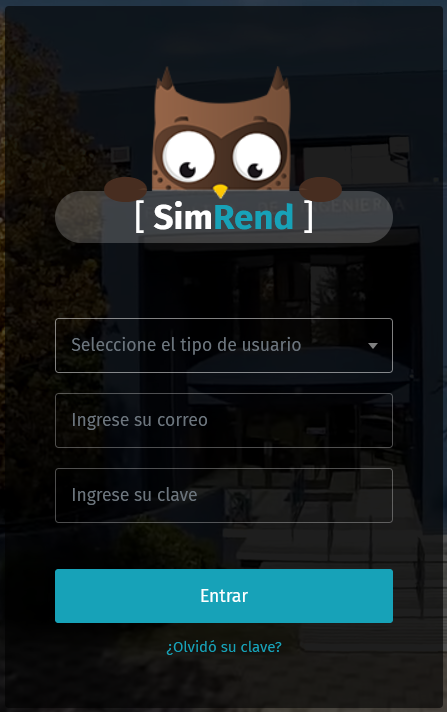
\includegraphics[width=0.35\textwidth]{Imagenes/Login.PNG}
    \caption{\label{fig: Login}Vista de ingreso al sistema.}
\end{figure}

\paragraph{Recuperación de acceso a una cuenta de una OE: } Solicitud de una nueva clave de acceso en caso de que el usuario la olvide, ingresando el correo su cuenta registrada. Una vez validada esta información se solicita la recuperación de cuenta al servidor, el cual envía un correo con la nueva clave de acceso al usuario (vea \textbf{Figura \ref{fig: RecuperarClave}}).

\begin{figure}[htbp]
    \centering
    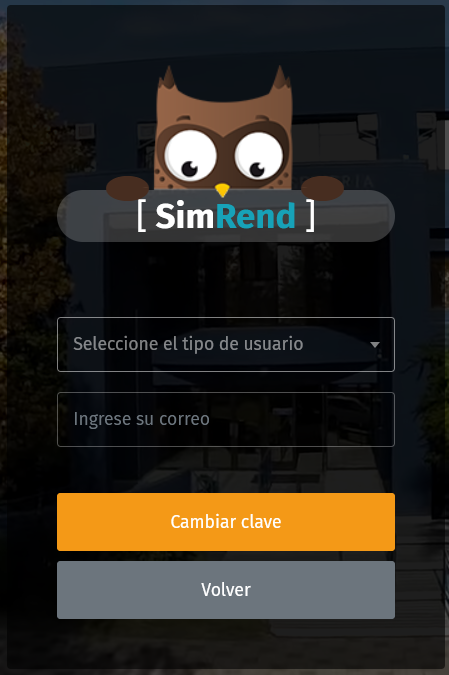
\includegraphics[width=0.35\textwidth]{Imagenes/RecuperarClave.PNG}
    \caption{\label{fig: RecuperarClave}Vista de recuperar clave.}
\end{figure}

\paragraph{Búsqueda de solicitudes: } En esta etapa de la aplicación se encuentran todas las solicitudes realizadas por la OE, en donde el usuario puede visualizar los resúmenes de la solicitudes y tener la opción de ver en detalle cada una de ellas. Además, se encuentra la opción de realizar búsquedas de solicitudes a través del nombre o la fecha del evento (vea \textbf{Figura \ref{fig: Busquedas}}). Esta funcionalidad de la aplicación ayuda a resolver el problema \textbf{PBLM-7}.

\begin{figure}[htbp]
    \centering
    \includegraphics[width=1\textwidth]{Imagenes/Busqueda.PNG}
    \caption{\label{fig: Busquedas}Vista de búsqueda de solicitudes.}
\end{figure}

\paragraph{Solicitud: }Esta etapa consta de 4 fases las cuales ayudan a la confección de la solicitud a presentar a la Dirección correspondiente de cada OE. Estas fases se detallan a continuación. Esta funcionalidad de la aplicación ayuda a resolver el problema \textbf{PBLM-7} y \textbf{PBLM-9}.

    \subparagraph{\emph{Datos principales de la Solicitud: }} Formulario que solicita el nombre, fecha de inicio, fecha de término, lugar y monto del evento, el responsable a cargo de la solicitud y la cantidad de participantes, la cual puede ser para un grupo de personas específico o masivo (e indeterminado), según sea el caso (vea \textbf{Figura \ref{fig: DatosPrincipales}}).

    \begin{figure}[htbp]
        \centering
        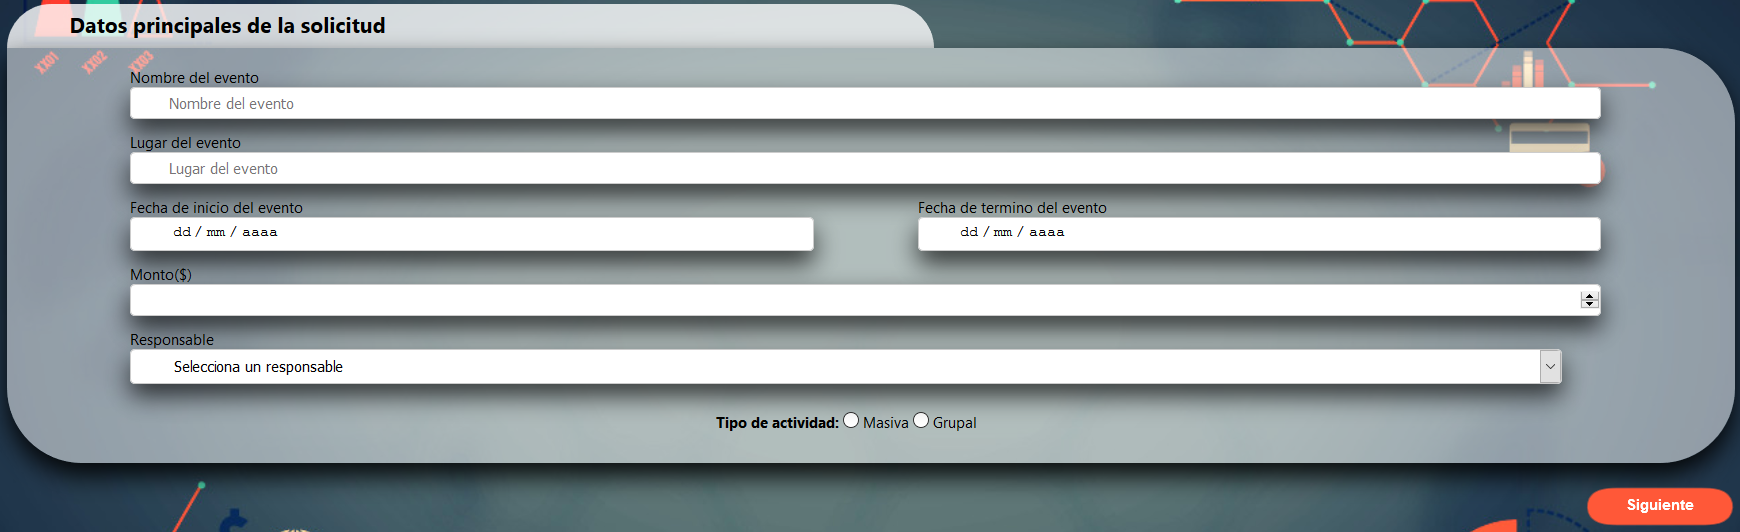
\includegraphics[width= 0.8\textwidth]{Imagenes/DatosPrincipales.PNG}
        \caption{\label{fig: DatosPrincipales}Vista que obtiene los datos principales de una Solicitud.}
    \end{figure}

    \subparagraph{\emph{Categoría: }} En esta etapa se solicitan todas las categoría de los gastos que se realizan dentro del evento para el cual se está realizando la solicitud (vea \textbf{Figura \ref{fig: Categorias}}).

    \begin{figure}[htbp]
        \centering
        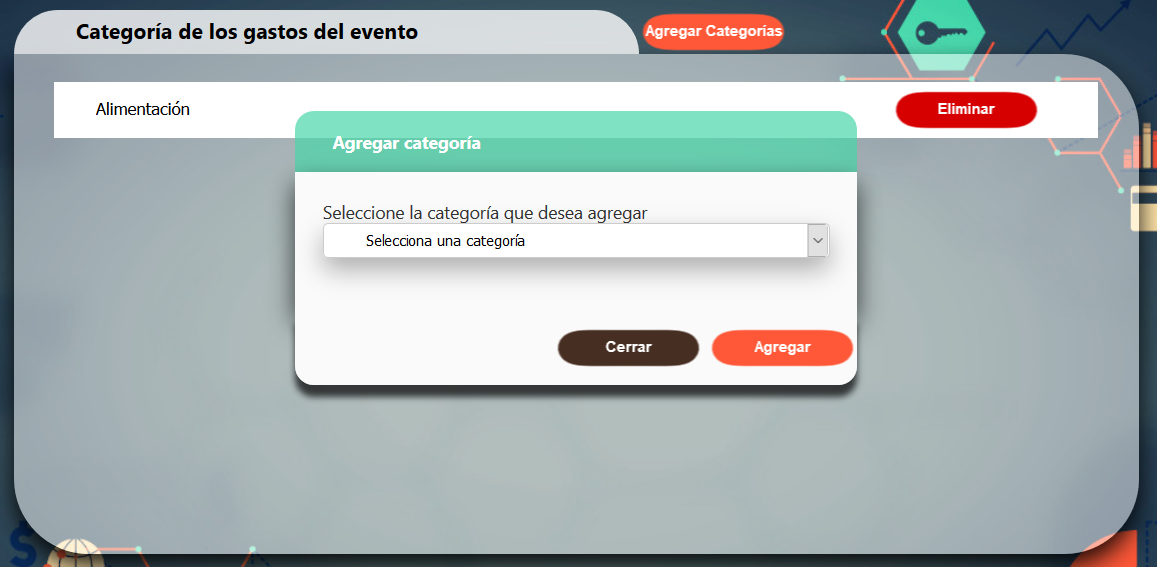
\includegraphics[width= 0.8\textwidth]{Imagenes/Categoria.PNG}
        \caption{\label{fig: Categorias}Vista que obtiene las categorías en que incurren los gastos.}
    \end{figure}

    \subparagraph{\emph{Participante: }} Formulario que solicita el nombre y RUT de los participantes de la actividad. Esta vista sólo se visualiza si en la etapa de \textbf{Datos principales de la solicitud} se indica que es para un grupo de personas específico (vea \textbf{Figura \ref{fig: Personas}}). Esta funcionalidad de la aplicación ayuda a resolver el problema \textbf{PBLM-3}.

    \begin{figure}[htbp]
        \centering
        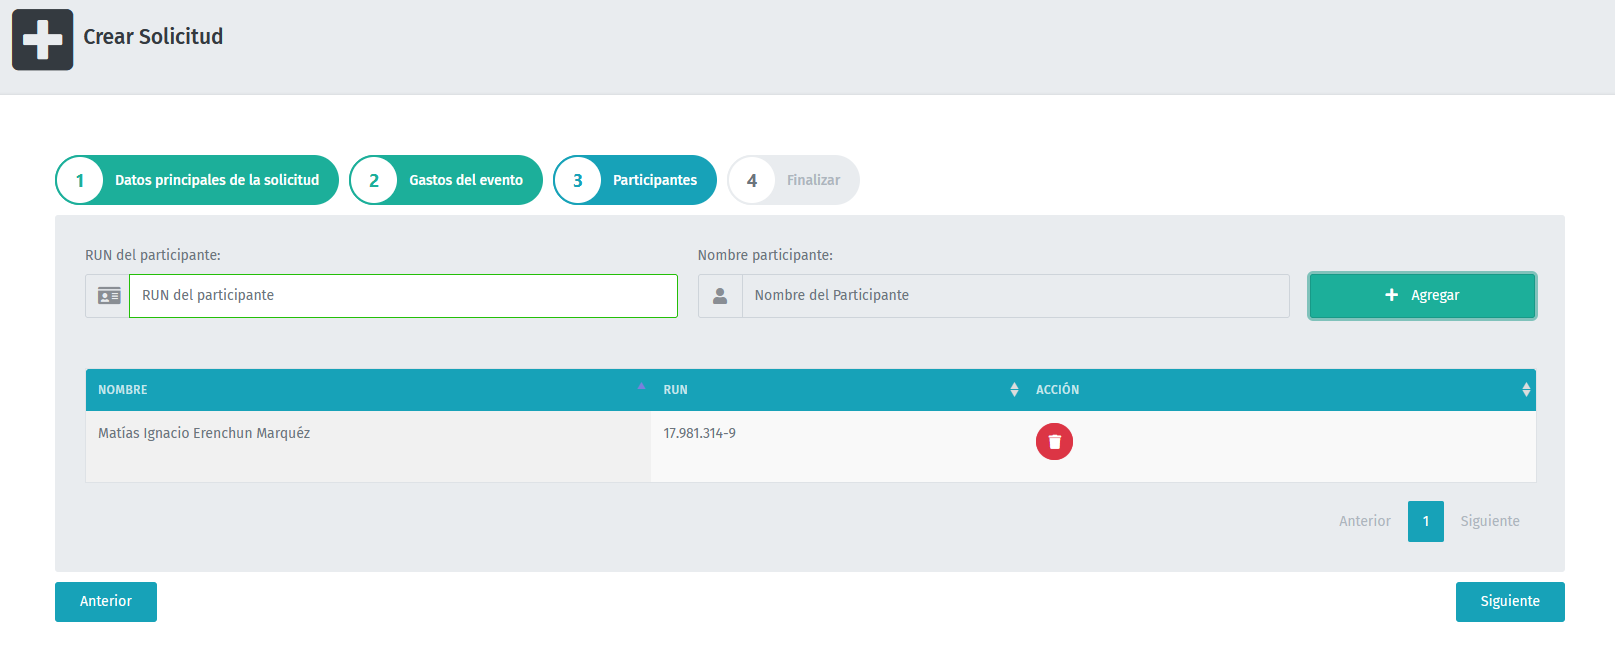
\includegraphics[width= 1\textwidth]{Imagenes/AgregarPersonas.PNG}
        \caption{\label{fig: Personas}Vista que obtiene los datos de los participantes del evento.}
    \end{figure}

    \subparagraph{\emph{Resumen: }} Etapa que muestra los datos principales de la solicitud y a su vez da la opción de generar el PDF de la solicitud (vea \textbf{Figura \ref{fig: ResumenSolicitud}}).

    \begin{figure}[htbp]
        \centering
        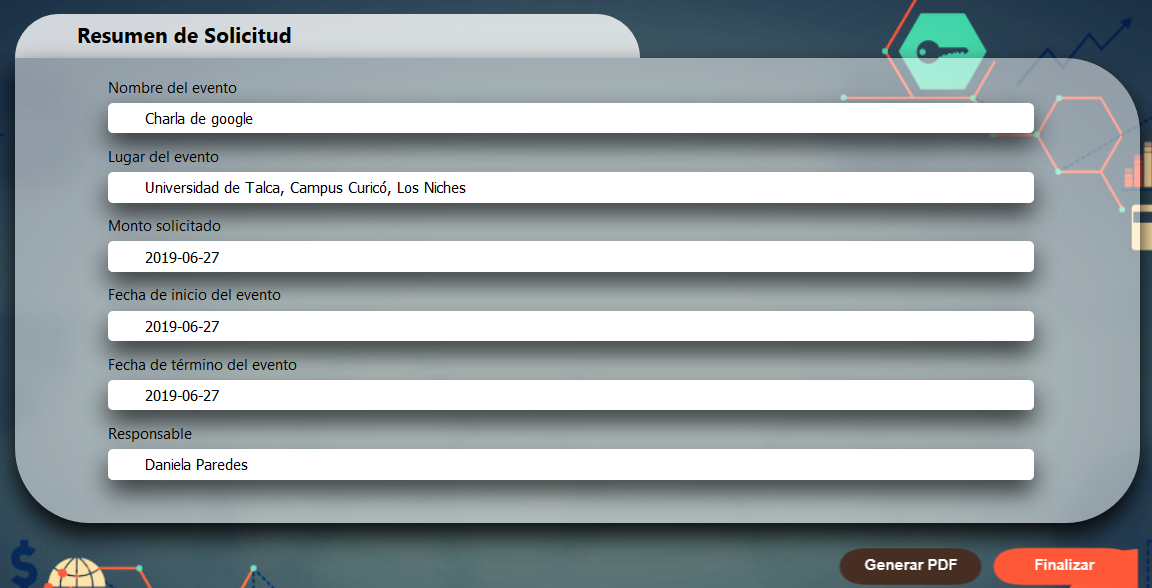
\includegraphics[width= 0.8\textwidth]{Imagenes/Resumen.PNG}
        \caption{\label{fig: ResumenSolicitud}Vista que muestra el resumen de los datos ingresados para la solicitud.}
    \end{figure}

\paragraph{Resolución: } En esta etapa se acepta o rechaza la solicitud. En caso de ser aceptada se procede a ingresar los datos principales de la RU enviada por la Casa de Estudios a la OE interesada, los cuales son el número de la resolución y el año de creación. Además, se solicita que se adjunte una copia digitalizada y en formato PDF de la RU correspondiente a la aceptación de la Solicitud enviada por la OE (vea \textbf{Figura \ref{fig: Resolucion}}). Esta funcionalidad de la aplicación ayuda a resolver el problema \textbf{PBLM-7}.

\begin{figure}[htbp]
    \centering
    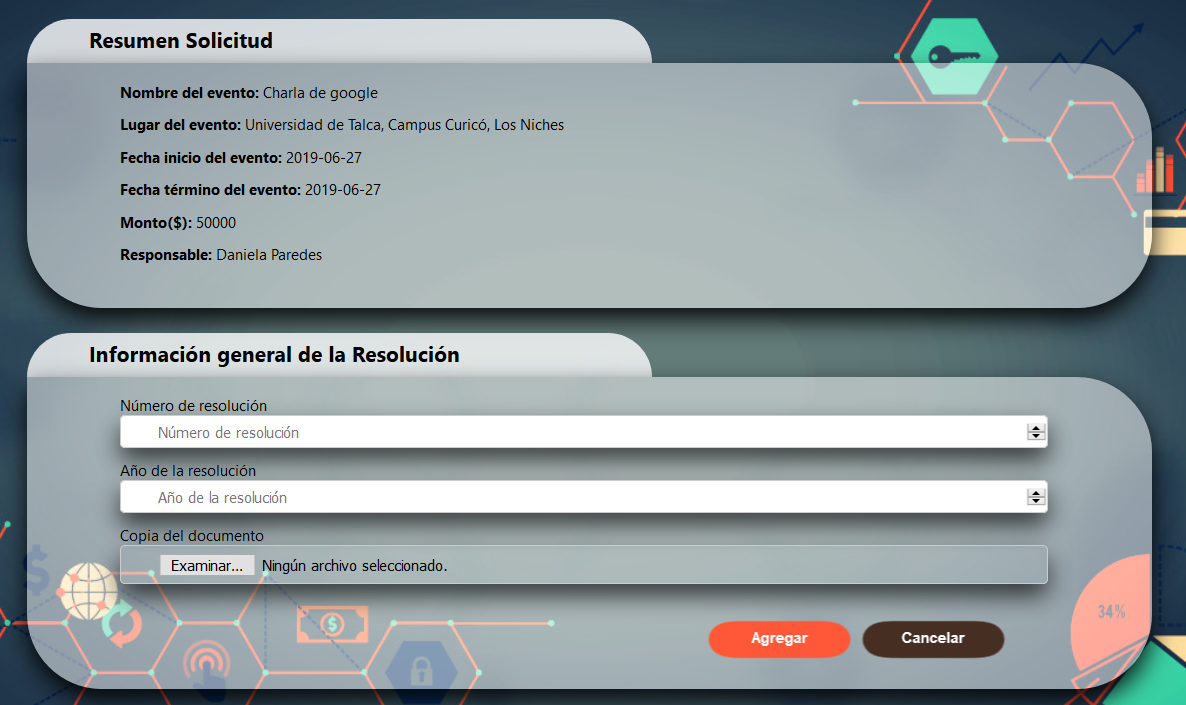
\includegraphics[width= 0.8\textwidth]{Imagenes/Resolucion.PNG}
    \caption{\label{fig: Resolucion}Vista que muestra el resumen de los datos ingresados para la solicitud y obtiene los datos principales de la RU.}
\end{figure}

\paragraph{Rendición: } Tras la aceptación de la Solicitud y el ingreso de los datos de la RU que la aprueba, se procede a realizar la Rendición correspondiente al evento. Si bien los datos principales de la Rendición tales como el nombre de la organización, el número de la resolución y el responsable del evento, entre otros, se obtiene automáticamente de los datos registrados en el sistema, el monto total rendido tiene dependencia del registro de documentos (boletas y/o facturas) (vea \textbf{Figura \ref{fig: Rendicion}}). Una vez finalizado el proceso de Rendición, está la opción de generar el documento a presentar obedeciendo el formato exigido por la casa de estudio. Esta funcionalidad de la aplicación termina de solucionar los problemas \textbf{PBLM-1}, \textbf{PBLM-2}, \textbf{PBLM-3} \textbf{PBLM-4}, \textbf{PBLM-7} y \textbf{PBLM-8}.

\begin{figure}[htbp]
    \centering
    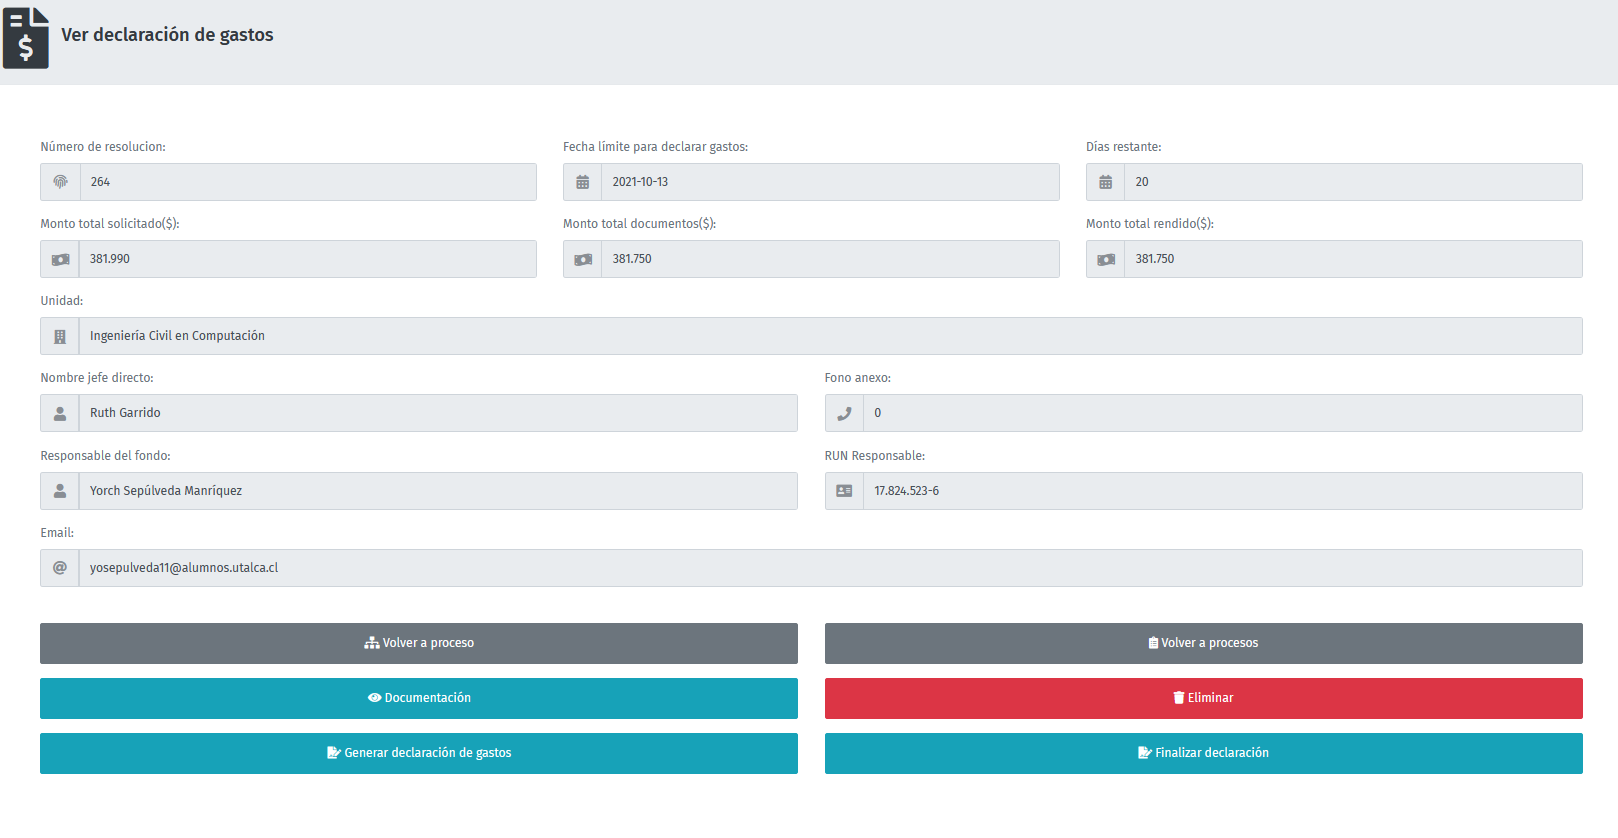
\includegraphics[width= 0.8\textwidth]{Imagenes/Rendicion2.png}
    \caption{\label{fig: Rendicion}Vista que muestra los datos principales de una Rendición.}
\end{figure}

    \subparagraph{\emph{Resumen de los gastos realizados por personas: }} Cuando el tipo de evento ingresado en la Solicitud está destinada a un grupo de personas, se debe declarar los gastos de cada uno de ellos y los gastos que han tenido en común. Es por ello que antes de ingresar la documentación, se muestra un resumen de los registros de documentos (vea \textbf{Figura \ref{fig: RendicionPersonas}}). Esta funcionalidad de la aplicación ayuda a resolver el problema \textbf{PBLM-3}.

    \begin{figure}[htbp]
        \centering
        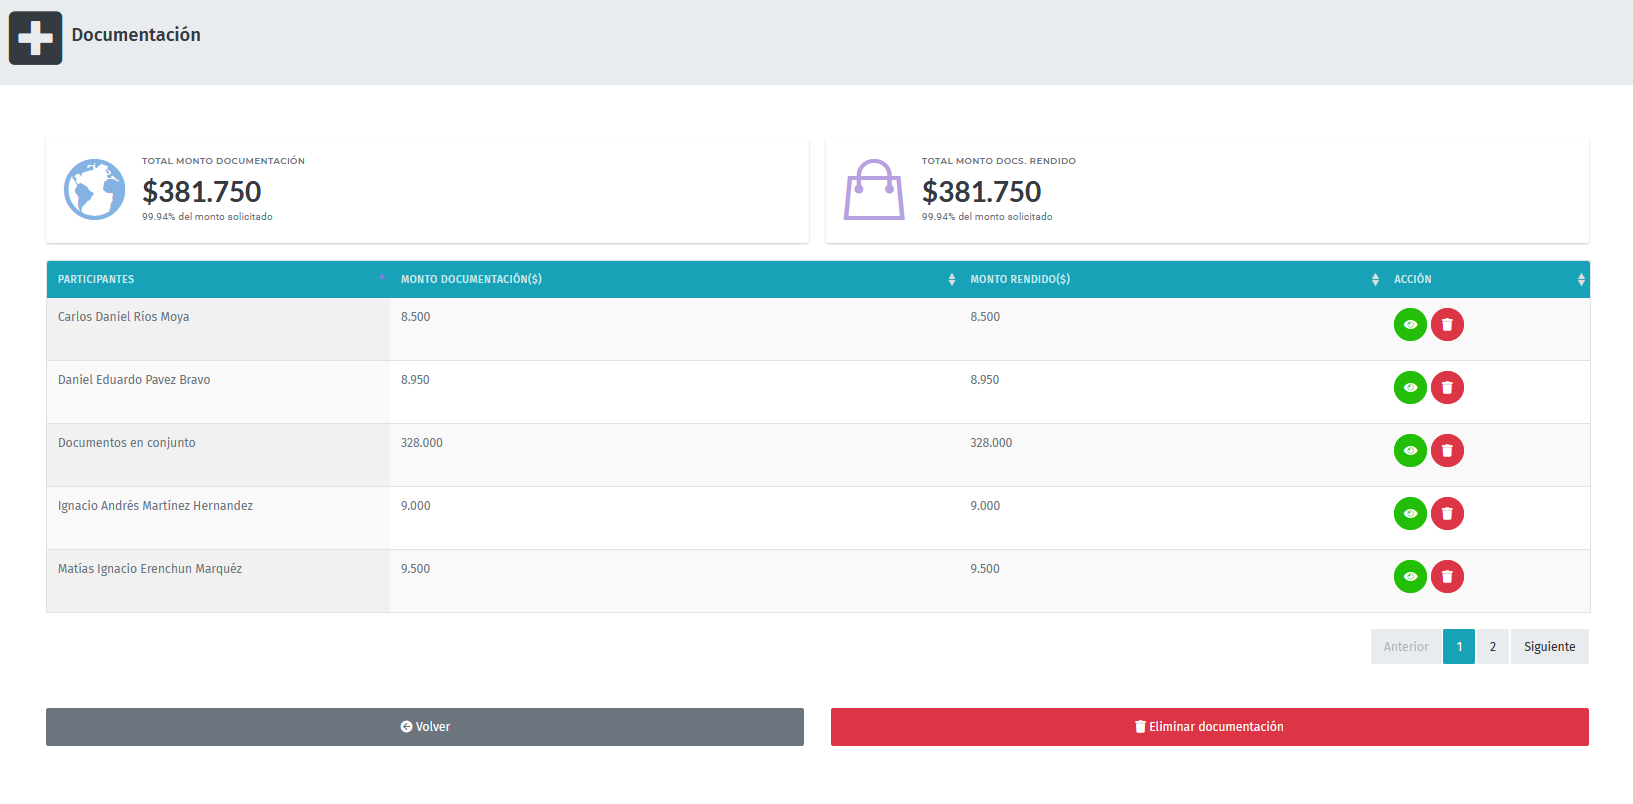
\includegraphics[width= 0.8\textwidth]{Imagenes/Rendicion_Personas2.PNG}
        \caption{\label{fig: RendicionPersonas}Vista que muestra el resumen de los documentos declarados por cada participante y los gastos comunes.}
    \end{figure}

    \subparagraph{\emph{Documentos de una persona: }} Tras seleccionar a la persona en el \textit{Resumen de los gastos realizados por personas} se procede a mostrar en detalle los documentos que se han registrado de esta y, además se muestran indicadores que ayudan a analizar cuanto es la suma total de los documentos registrados para la declaración de gasto, cuanto es la suma total de los documentos seleccionados a rendir, cuanto es la suma de los documentos registrado para declarar del participante y cuanto es la suma de los documentos que se han seleccionado para declarar del participante (vea \textbf{Figura \ref{fig: DocumentosParticipante}}). Esta funcionalidad de la aplicación ayuda a resolver el problema \textbf{PBLM-3}.

    
    \begin{figure}[htbp]
        \centering
        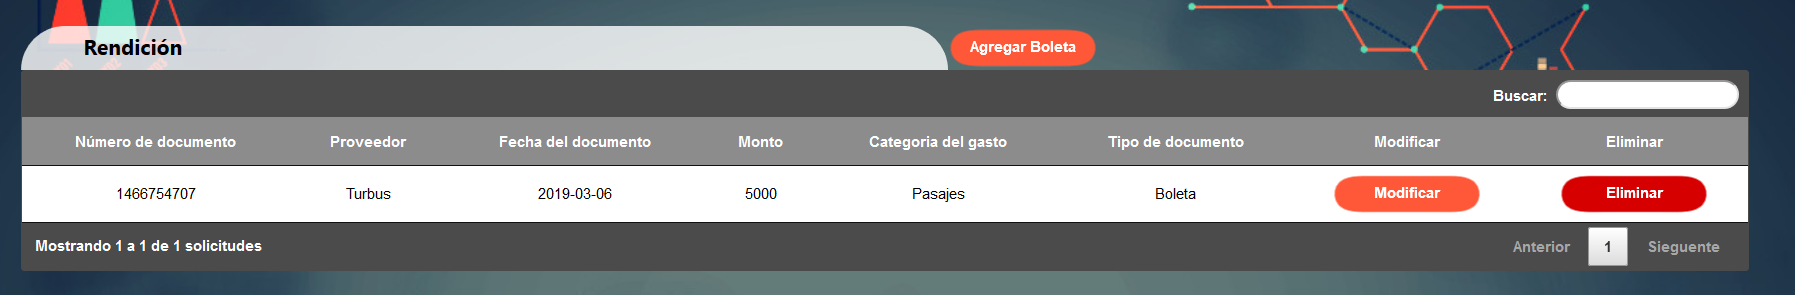
\includegraphics[width= 0.8\textwidth]{Imagenes/Boletas_de_un_participante.PNG}
        \caption{\label{fig: DocumentosParticipante}Vista que muestra en detalle los documentos registrados que ha presentado un participante cuya actividad ingresada en la solicitud es de tipo grupal.}
    \end{figure}

    
    \subparagraph{\emph{Documento: }} Sección en donde se ingresan los datos de una boleta y/o factura, que corresponden al número del documento, la categoría en que incurrieron los gatos, la fecha de compra de los productos, el monto, una pequeña descripción de los gastos y el proveedor, entre otros (vea \textbf{Figura \ref{fig: AgregarBoletas}}). Esta funcionalidad de la aplicación ayuda a resolver los problema \textbf{PBLM-4} y \textbf{PBLM-6}.

    \begin{figure}[htbp]
        \centering
        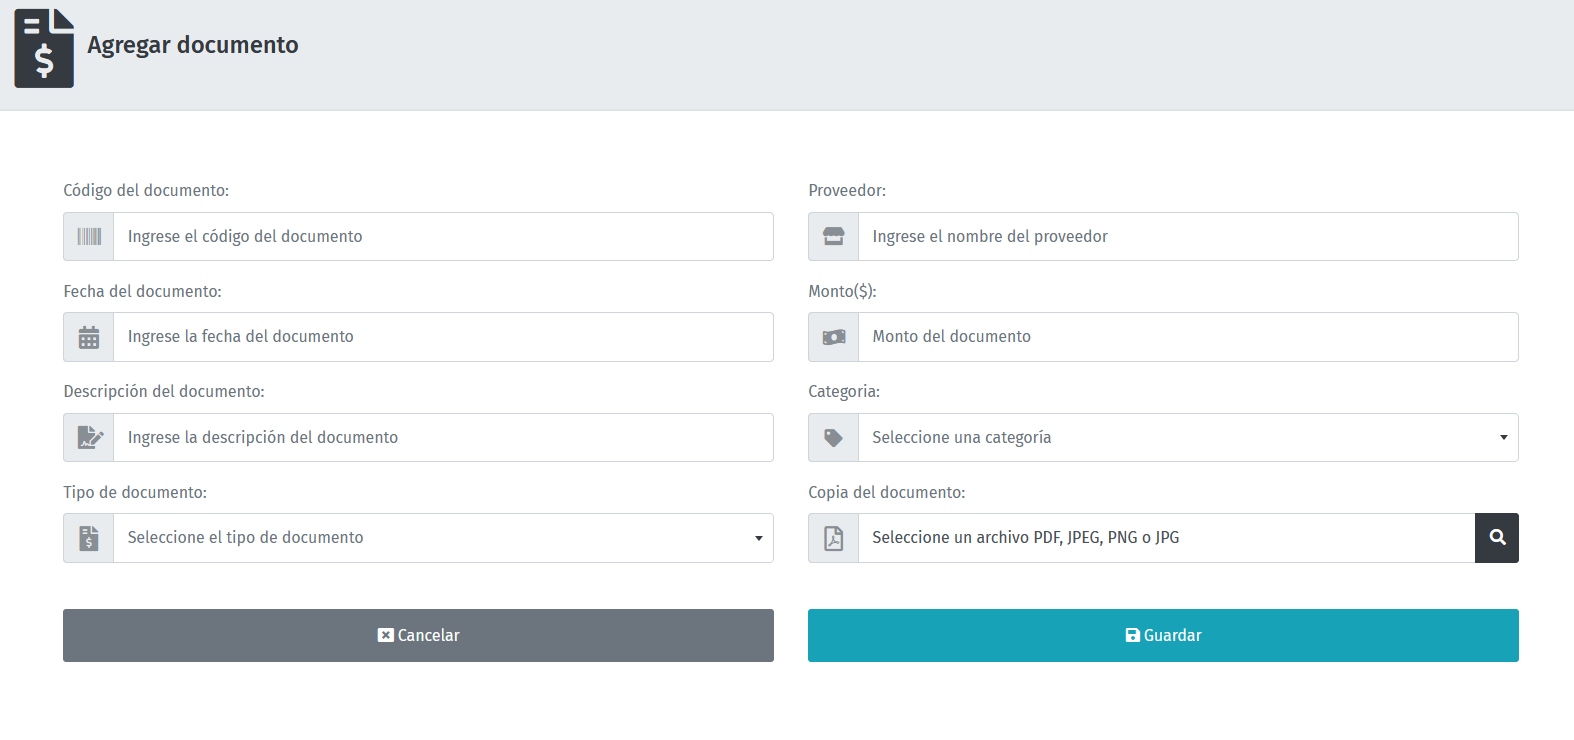
\includegraphics[width= 0.8\textwidth]{Imagenes/AgregarBoletas.PNG}
        \caption{\label{fig: AgregarBoletas}Vista que obtiene los datos de una boleta o factura.}
    \end{figure}

    \subparagraph{\emph{Aceptar o Rechazar una Rendición: }} Una vez finalizada la Rendición, la aplicación queda a espera de que la Universidad notifique la aceptación o el rechazo de esta. En caso de que se acepte, el proceso finaliza. Mientras que si se rechaza, la aplicación da un plazo de 20 días corridos para modificar la Rendición y su posterior envío al Depto. de Tesorería y Presupuesto (vea \textbf{Figura \ref{fig: AceptarRechazarDG}}).

    \begin{figure}[htbp]
        \centering
        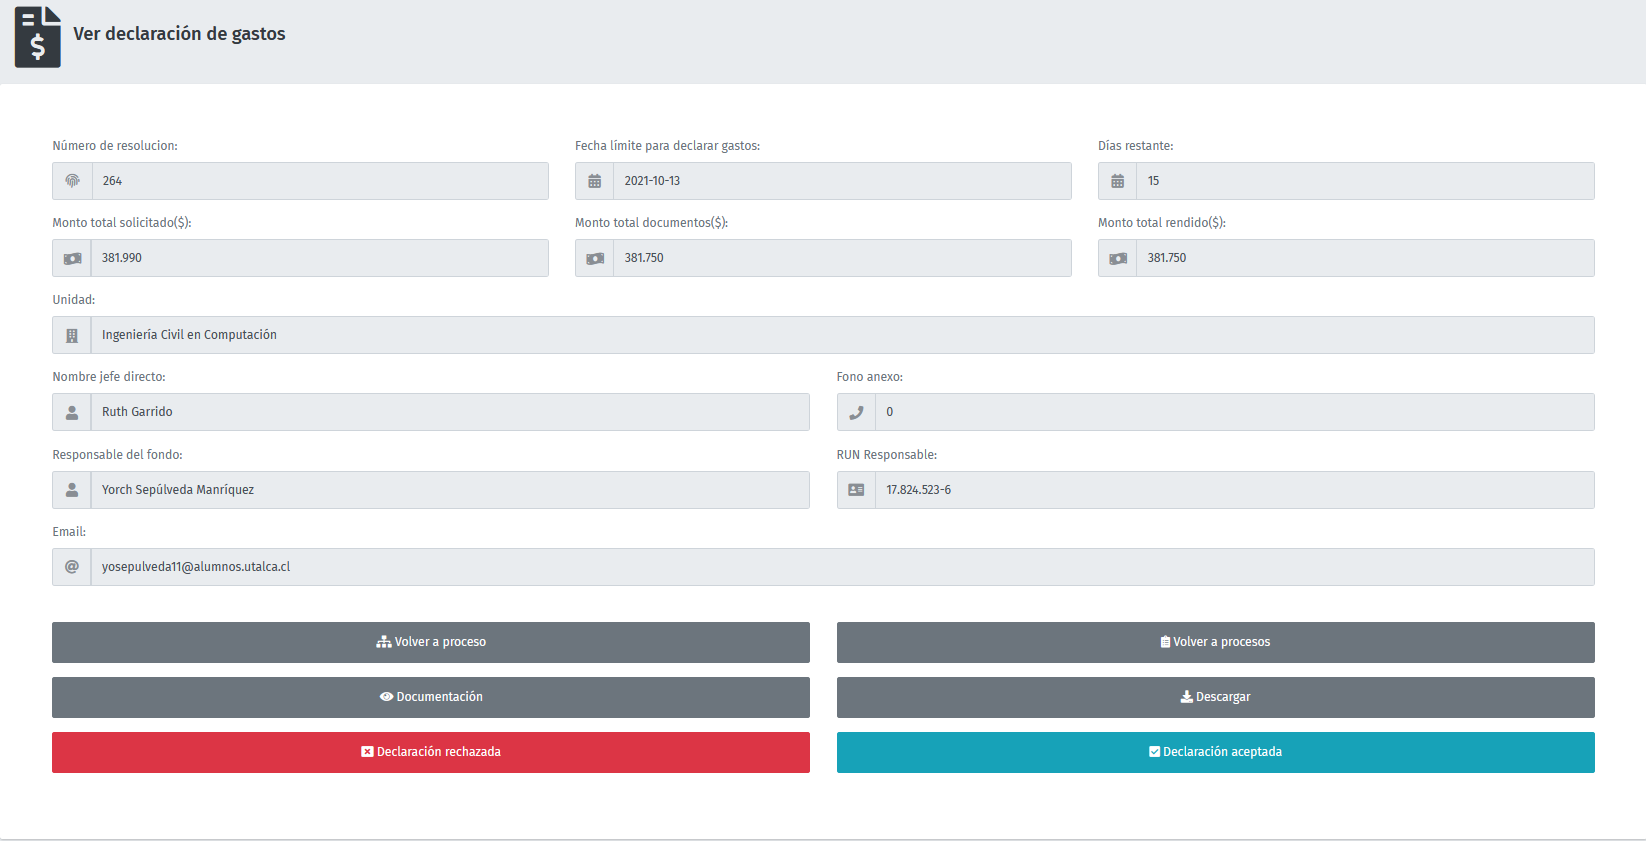
\includegraphics[width= 0.8\textwidth]{Imagenes/AceptarRechazarDeclaracion.PNG}
        \caption{\label{fig: AceptarRechazarDG}Tras finalizar la Rendición, se habilitan las opciones de Aceptar o Rechazar, de acuerdo a lo que responda el Depto. de Tesorería y presupuesto.}
    \end{figure}



    \vspace{10mm}
    Tras lo mencionado con aterioridad se realiza el \textbf{Cuadro \ref{tab: Solucion_Problemas_Frecuentes}}, el cual representa en resumen la funcionalidad de la aplicación obtenida y el/los problema(s) que resuelve mencionados en la  \textbf{Sección \ref{sec:Errores_Frecuentes}}.


    \begin{table}[htbp]
        \centering
        \caption{Solución a problemas frecuentes}
        \label{tab: Solucion_Problemas_Frecuentes}
        \begin{tabular}{| p{7cm}| p{7.4cm} |}
        \hline
        \textbf{Nombre de la intefaz} & \textbf{Problema que soluciona} \\
        \hline \hline

        Búsqueda de solicitud & PBLM-7 \\ \hline

        Solicitud & PBLM-7 y PBLM-9\\ \hline

        Participante & PBLM-3 \\ \hline

        Resolución & PBLM-7 \\ \hline

        Rendición & PBLM-1, PBLM-2, PBLM-3 ,PBLM-4, PBLM-7 y PMBL-8 \\ \hline

        Resumen de los gastos realizados por personas & PBLM-3\\ \hline

        Documentos de una persona & PBLM-3\\ \hline

        Documento & PBLM-4 y PBLM-6\\ \hline
        \end{tabular}
    \end{table}
